\documentclass[10pt]{article}
\usepackage[letterpaper,landscape,margin=0.65in]{geometry}
\usepackage{graphicx}
\usepackage{booktabs}
\usepackage[T1]{fontenc}
\usepackage{hyperref}
\hypersetup{pdftitle={BINSTD runner source restoration with prior toy replay}}
\setlength{\parindent}{0pt}
\setlength{\parskip}{0.42em}
\title{BINSTD runner source restoration with prior toy replay}
\author{Validation audit, 22 October 2026}
\date{}
\begin{document}
\maketitle
\vspace{-2em}

\textbf{Finding.} On main \texttt{13eb21767865}, the BINSTD runner
accepts none of the \texttt{--ells}, \texttt{--artifact-tag} and
\texttt{--seed} options used by the archived Stage-1 commands. The
current runner's SHA-256 begins \texttt{6d0e90f863c4}. The ell89
snapshot at \texttt{8efed7dea288} contains source hash
\texttt{7efcf8e6bbfc}; the ell89r1 snapshot at
\texttt{c39a3d5e4cc7} contains \texttt{17a3175a30b2}. Each matches
the corresponding frozen run environment. The field helper and checker
match both snapshots and current main.

\textbf{Correction.} The live \texttt{implementation/run.py} is now the
exact \texttt{c39a3d5e4cc7} runner. This restores both additive panels
and their CLI without altering a run or scientific record. The
source-custody receipt binds the snapshots, run environments and
restored file.

\textbf{Algebra check.} An independent SymPy factorization confirms
that $t^{17}+t^3+1$ is irreducible over $\mathbf F_2$ and that
$x^{17}+1$ has irreducible degrees $1,8,8$. The restored code builds
Frobenius-closed kernels of dimensions 8 and 9; dimensions 3 and 4
are excluded. Sampled curve equations, group associativity and
small-factor-base triple membership pass.
The full ledger validator still exits 1 with the same 141 errors
in 39 paths as main; the log is byte-for-byte unchanged.

\textbf{Prior replay.} An existing source-pinned audit already ran
both archived Stage-1 panels in temporary directories. Its receipt
records exact matches for both frozen dimension tables, yield matrices
and result notes, plus bounded independent arithmetic controls.
This patch restores that latest historical source to current main;
the completed full-panel replay was not repeated.

\textbf{Boundary.} The prior deterministic replay of the archived toy
algorithm is not an independent per-target relation proof or a Lean
yield theorem. It does not change the measured ratios, scoped
decisions, performance estimates or any deployed-curve claim.

\newpage
\begin{center}
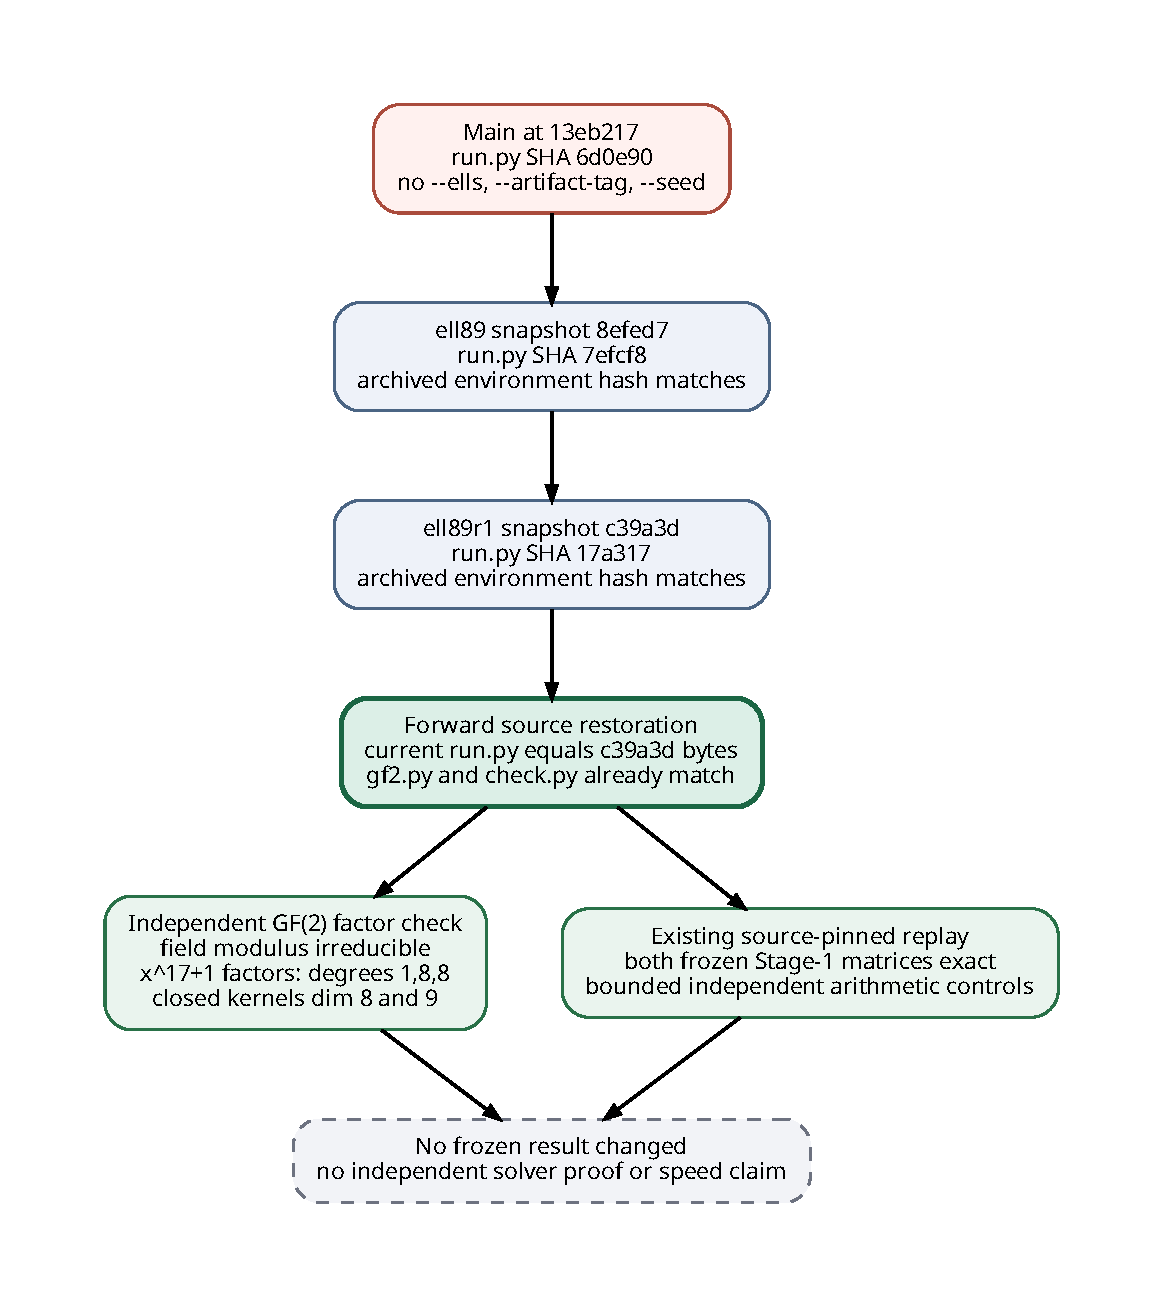
\includegraphics[width=\textwidth,height=0.82\textheight,keepaspectratio]{source-figure.pdf}
\end{center}
\end{document}
